\documentclass[aspectratio=169]{beamer}
\usetheme{Copenhagen}
%% Remove draft for real article, put twocolumn for two columns
\usepackage[utf8]{inputenc}

\newcommand{\vectorproj}[2][]{\mathrm{proj}_{\vect{#1}}\vect{#2}}
\newcommand{\vectorcomp}[2][]{\mathrm{comp}_{\vect{#1}}\vect{#2}}
\newcommand{\vect}{\mathbf}
%% commentary bubble
\newcommand{\SV}[2][]{\sidenote[colback=green!10]{\textbf{SV\xspace #1:} #2}}

%% Title 
\title{ Multivariable Calculus \\ Day 1}
\institute{Fulbright University Vietnam}
%\author[1]{Co-author}
\author{Truong-Son Van}
\date{Spring 2024}

\begin{document}

\maketitle


\begin{frame}
    \frametitle{Introduction}
    \begin{itemize}
        \item Instructor: Truong-Son Van
        \item Time: M \& W, 9:45a-11:15a
        \item Office hours: TBD 
        \item TA:  TBD
    \end{itemize}
\end{frame}

\begin{frame}
    \frametitle{Overview}
    \begin{itemize}
        \item Logistics
        \item Getting started with linear algebra
    \end{itemize}
\end{frame}

\begin{frame}
    \frametitle{Single variable vs. Multivariable}

\end{frame}

\begin{frame}
    \frametitle{What's the point?}
    What do you think is the function that create this graph?
    \centering
    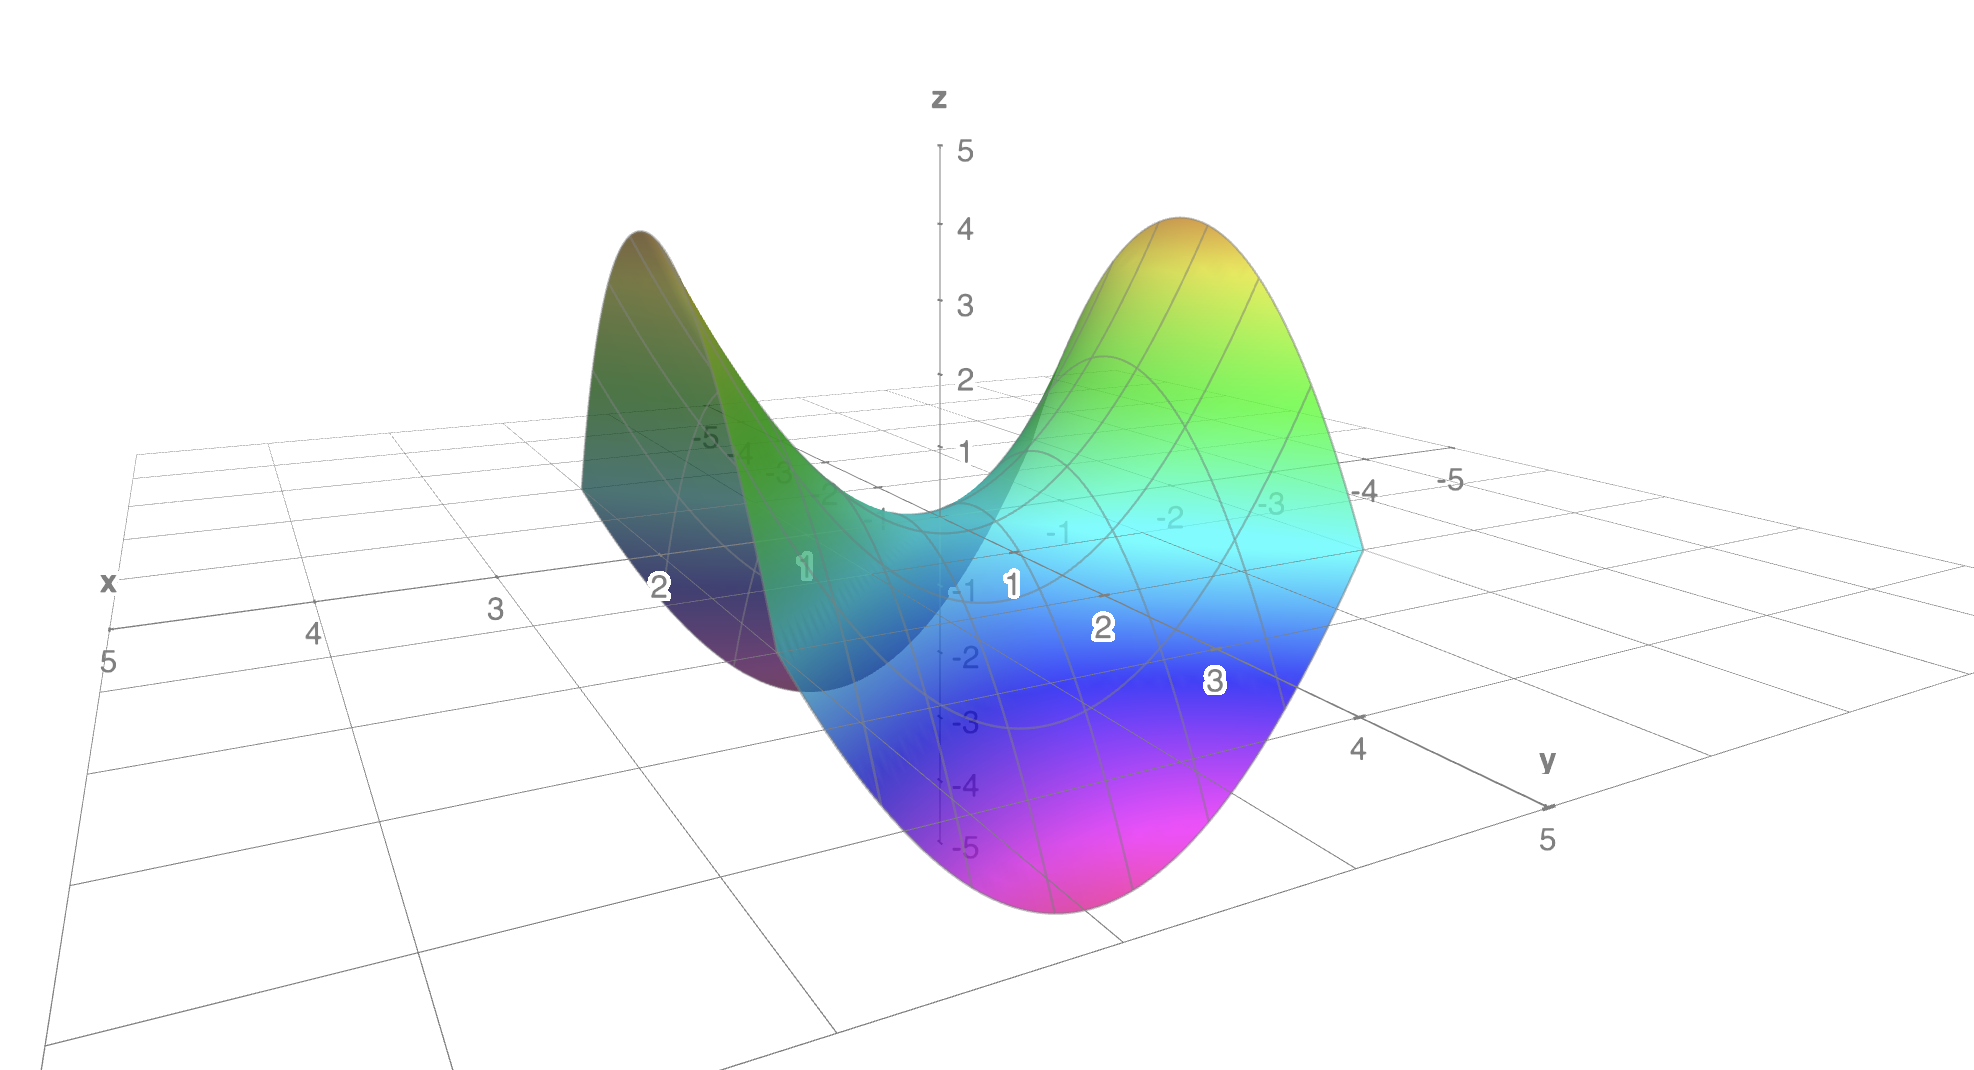
\includegraphics[width=0.7\textwidth]{saddle}
\end{frame}

\begin{frame}
    \frametitle{What's the point?}
    Life is a function with many variables \pause

    \centering
    
\includegraphics[height=0.5\textheight]{sad}
\end{frame}

\begin{frame}
    \frametitle{What will you learn?}
    \url{https://www.tsvan.xyz/MultiCalc/\#core-content}
\end{frame}


\begin{frame}
    \frametitle{Assessment}
    \begin{itemize}
        \item Homework (40\%)
        \item Quizzes(10\%)
        \item Midterm (20\%)
        \item Final (30\%)
    \end{itemize}
\end{frame}

\begin{frame}
    \centering
    DON'T CHEAT!!!
\end{frame}

\begin{frame}
    \frametitle{Final word on style}
    \begin{itemize}
        \item Certain things in math have to be delivered while writing.
        \item So, I'll deliver my lectures by writing on the iPad / whiteboard.
        \item Slides/brief notes just contain key points.
        \item It is your responsibility to update your notes to include the details I speak in class.
    \end{itemize}



\end{frame}

\begin{frame}
    \frametitle{Crash course in linear algebra}
    First, we need some language from linear algebra. 
\end{frame}

\begin{frame}
    \frametitle{Vectors}

    \begin{definition}
    An \(n\)-dimensional Euclidean space \(\mathbb{R}^n\)
    is the Cartesian product of \(n\) Euclidean spaces \(\mathbb{R}\).
    \end{definition}

    \begin{definition}
    An \(n\)-dimensional vector \(\textbf{v}\in \mathbb{R}^n\) is a tuple
    \begin{equation}
        \textbf{v} = \langle v_1,\dots, v_n \rangle \,,
    \end{equation}
    where \(v_i \in \mathbb{R}\).
    \end{definition}

    In dimensions less than or equal to 3, we represent a vector
    geometrically by an arrow, whose length represents the magnitude.
\end{frame}

\begin{frame}
    \frametitle{Examples}
    \begin{itemize}
        \item Vector connecting two points $(1,2)$ and $(4,5)$ in $\mathbb{R}^2$
        \item Zero vector
        \item Unit vector
    \end{itemize}
\end{frame}

\begin{frame}
    \frametitle{Worksheet}
    \begin{itemize}
        \item Write the general formula for a vector that connects
            any two points $A$ and $B$ in $\mathbb{R}^n$.
    \end{itemize}
\end{frame}


\begin{frame}
    \frametitle{Rules to manipulate vectors}

Let \(\textbf{a}, \textbf{b} \in \mathbb{R}^n\) and \(c,d \in \mathbb{R}\). Then,

\begin{equation*}
    c( \textbf{a} + \textbf{b}) = \langle c a_1 + c b_1, \dots, c a_n + c b_n \rangle  
    = c\textbf{a} + c\textbf{b} \,,
\end{equation*}
and
\begin{equation*}
 (c+d) \textbf{a} = c\mathbf{a} + d\mathbf{a} \,.
\end{equation*}

\end{frame}

\begin{frame}
    \frametitle{Worksheet}
    \begin{itemize}
        \item Elementary vectors have the form
    $$ \vect{e_i} = \langle 0, \dots, 1,  \dots, 0\rangle \,.$$
    Express a vector $\vect{u} \in \mathbb{R}^n$ in terms of these elementary vectors.
        \item In 3D,
    \begin{equation*}
        \vect{e_1} = \vect{i} \,, \qquad 
        \vect{e_2} = \vect{j} \,, \qquad
        \vect{e_3} = \vect{k} \,.
    \end{equation*}
    Write the vector connecting $A(1,2,3)$ with $B(-10,-3,5)$ in terms of elementary vectors.
    \end{itemize}
\end{frame}

\begin{frame}
    \frametitle{Geometric meanings}
\end{frame}


\end{document}
